% !TeX root = ../Rules.tex
% !TeX spellcheck = en_US
\section{Environment}
\label{sec:environment}

\subsection{The Field of Play}
\label{sec:field}

% ADDED BY REINALDO

The competition consists of three distinct divisions, categorized specifically by the maximum physical height and weight of the robotic platforms.

To ensure a fair and proportionate competitive environment, the field dimensions, number of players and ball size will vary to align with the specific requirements of each division\footnote{Games are played in three divisions depending on weight and height of the robots. See \ref{sec:divisions} for more details.}.

\subsubsection{Field surface}
\label{sec:field_surface}
The matches are played on artificial turf with a height of approximately 30 mm, except for the small division, which has a height of approximately 8 mm. \info{to be decided}

The color of artificial turf must be green. No particular shade is required, but the green must contrast well with the field markings and the ball and should not be very dark.

\subsubsection{Field markings}
\label{sec:field_markings}

The field of play must be rectangular and marked with continuous lines.
These lines belong to the areas of which they are boundaries.

The color of field markings should be white, whether applied by tape, paint, or made from white turf.

The two longer boundary lines are called touch lines. The two shorter lines are called goal lines.

The field of play is divided into two halves by a halfway line, which joins the midpoints of the two touch lines.

The center mark is at the midpoint of the halfway line. A circle is marked around it. 

% Removed by Reinaldo
%The radius of the circle depends on the division; see Figure \ref{fig:field_dim}. \info{to be decided}

The goal area and penalty area are defined using lines drawn at right angles to the goal line.

All lines must be of the same width, which must be approximately 5 cm.

Figure \ref{fig:field_line_names} shows the field markings with the lines and its names.

\begin{figure}[h]
    \centering
    \centerline{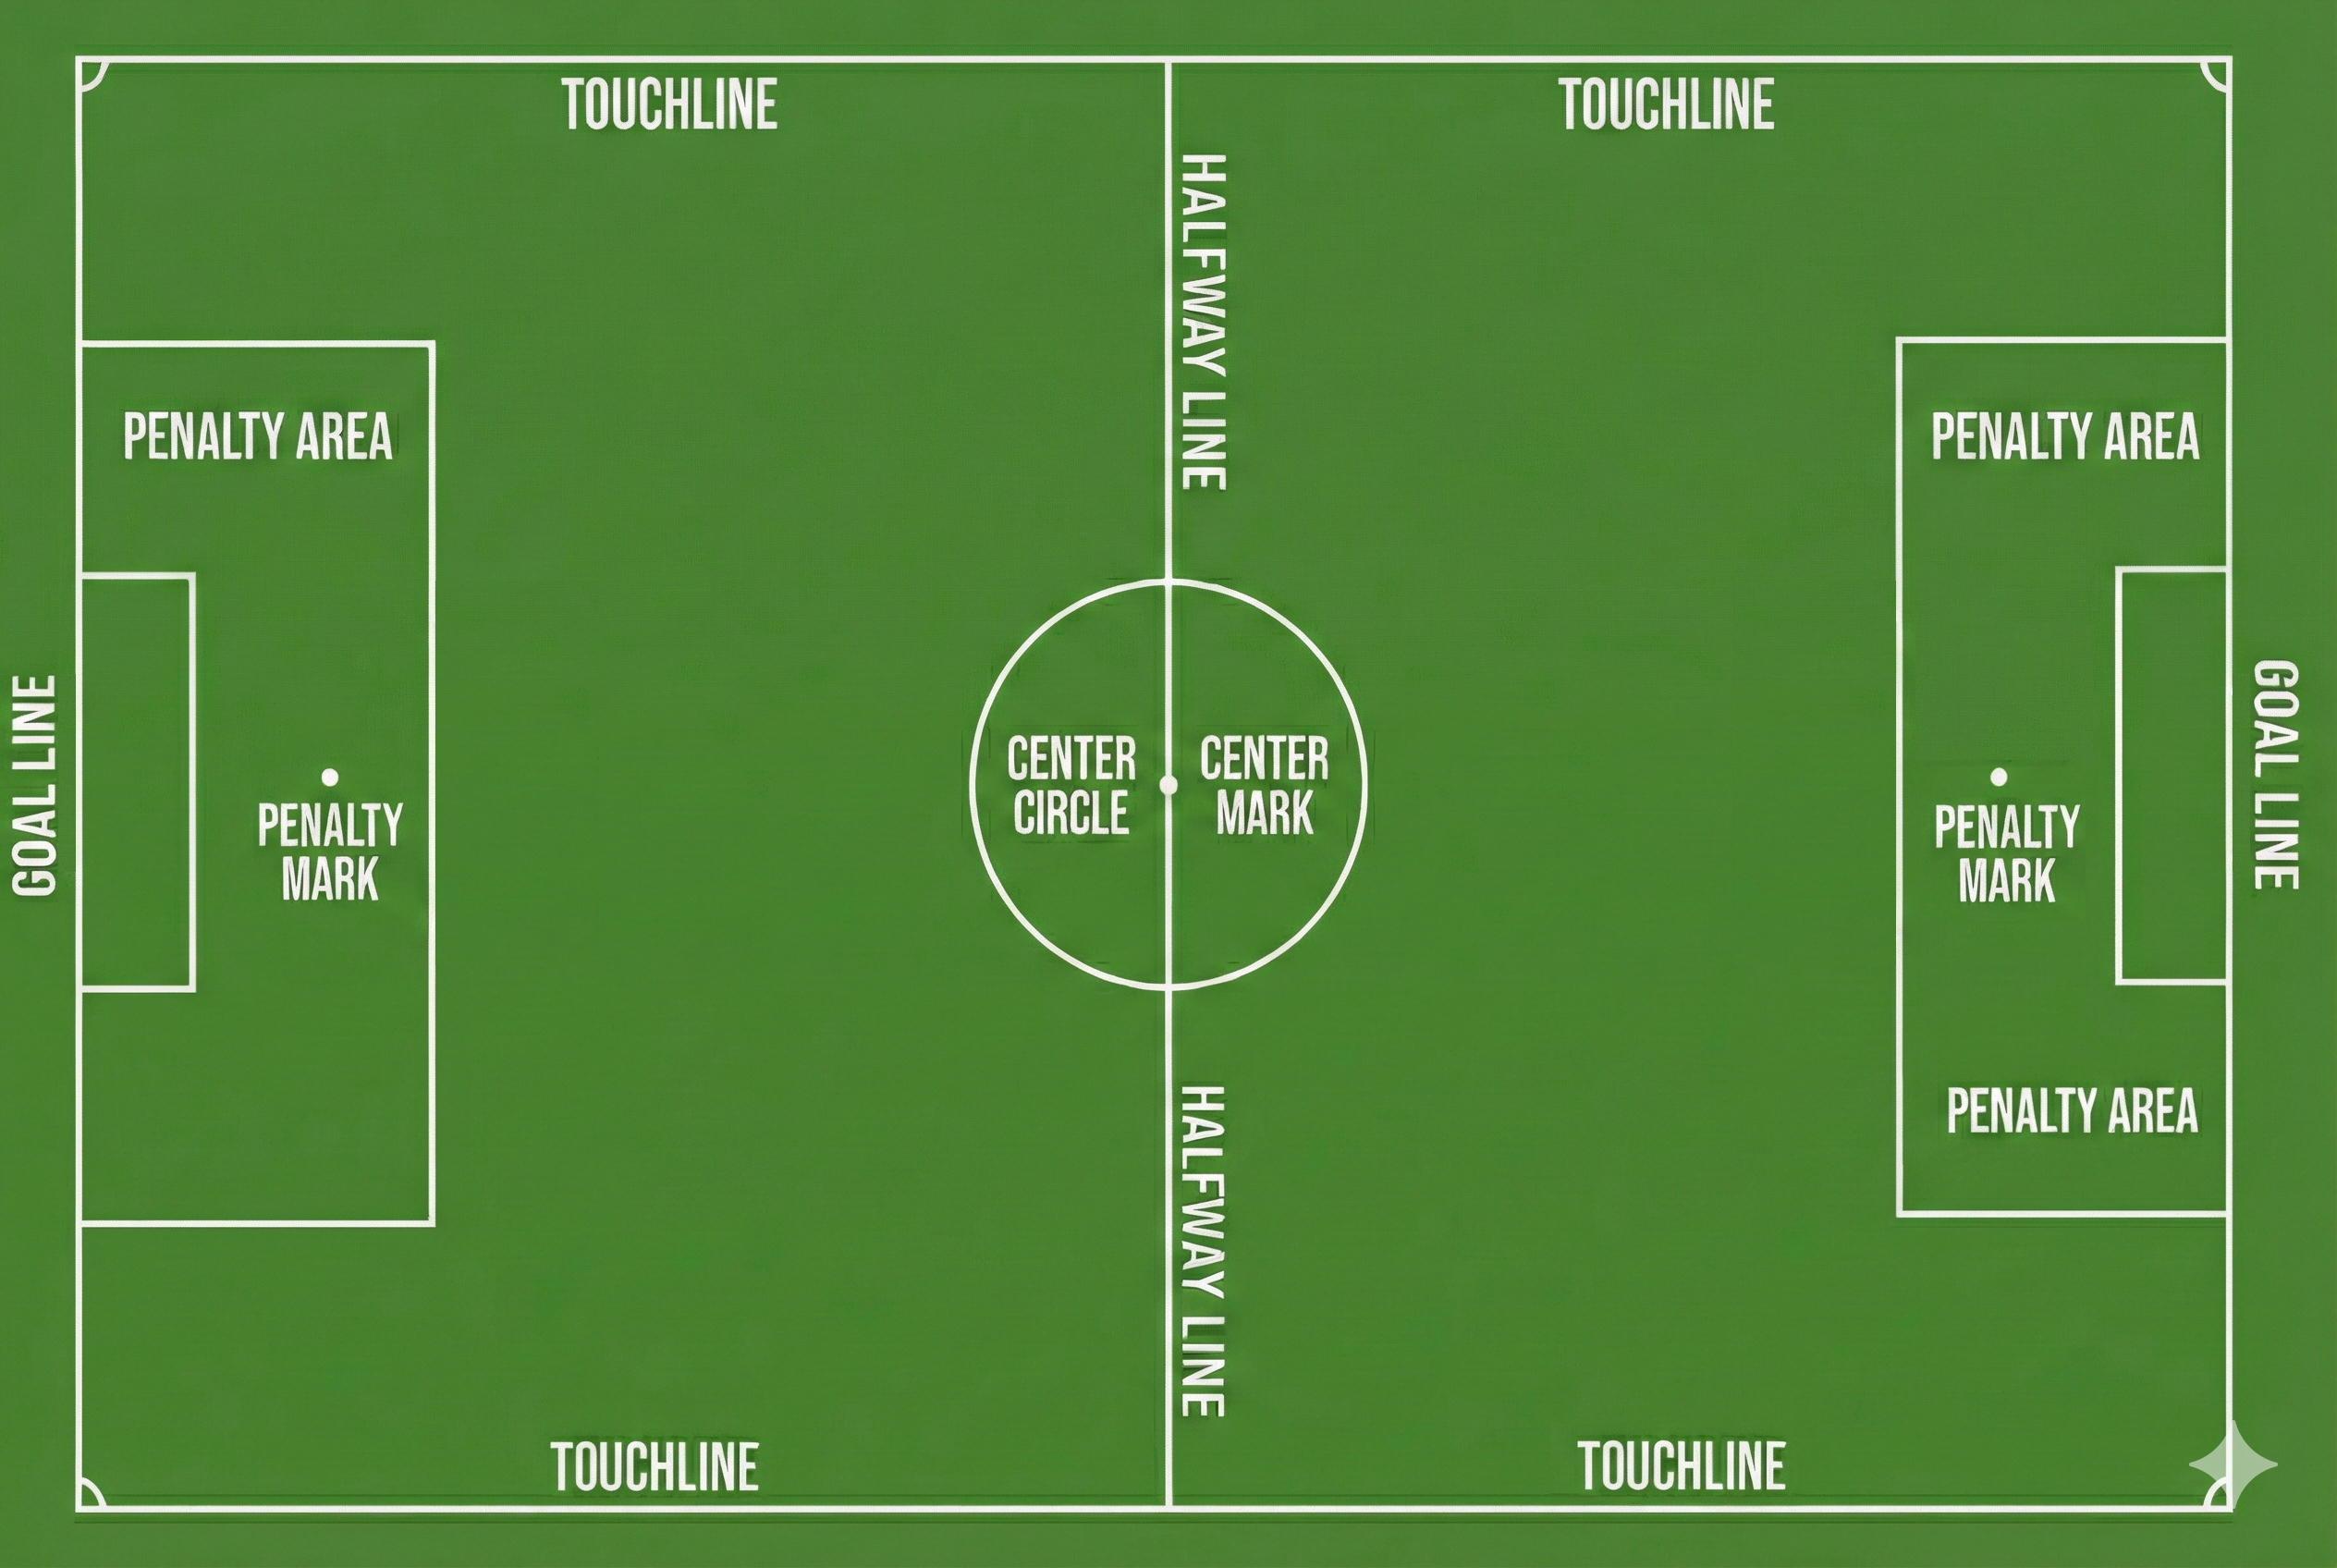
\includegraphics[width=0.7\columnwidth]{figs/Figure-1-line-names.png}}
    \caption{A labeled diagram illustrating the standard markings and key areas of a soccer field.}      
    \label{fig:field_line_names}
\end{figure}



\subsubsection{The goal area}
\label{sec:goal_area}
Two lines are drawn at right angles to the goal line; the length and distance from the midpoint of the goal line depend on the division.

These lines extend into the field of play and are joined by a line drawn parallel with the goal line.
The area bounded by these lines and the goal line is the goal area.

\subsubsection{The penalty area}
\label{sec:penalty_area}
Two lines are drawn at right angles to the goal line; the length and distance from the midpoint of the goal line depend on the division.

These lines extend into the field of play and are joined by a line drawn parallel with the goal line.
The area bounded by these lines and the goal line is the penalty area. 

Within each penalty area, a penalty mark is made. 

The distance from the midpoint between the goalposts depends on the division.

\subsubsection{Dimensions}
\label{sec:dimensions}


The touchline must be longer than the goal line.
%
% Removed by Reinaldo 
%\info{Note: Field dimensions for Middle / Large division are still subject to discussion.}

Figure \ref{fig:field_dim} shows the dimensions of the soccer fields and table \ref{table:field_dim} shows the dimensions depending on the division. More detailed technical drawings are provided in Section \ref{sec:technical_drawings}.

Note that measurements on this diagram are made to the center of lines (SPL Rule) OR Measurements are from the outside of the lines as the lines are part of the area they enclose (HL and FIFA Rule). \info{This needs to be decided}

\begin{figure}[h]
    \centering
    \centerline{\includegraphics[width=\columnwidth]{figs/field_simple.pdf}}
    \caption{Schematic diagram of the soccer field (not to scale).}      
    \label{fig:field_dim}
\end{figure}

\begin{center}
    \begin{table}[h]
        \centering
        \begin{tabular}{|l|l|c|c|c|}
            \hline
            ID & Description & S-Field & M-Field & L-Field (MSL) \\
            \hline \hline
            A & Field length & 9 m & 14 m & 22 m \\ 
            \hline
            B & Field width & 6 m & 9 m & 14 m \\ 
            \hline
            C & Line width & \multicolumn{2}{c|}{5 cm}& 12 cm\\
            \hline
            D & Penalty mark size & \multicolumn{2}{c|}{10 cm} & 15 cm\\
            \hline
            E & Goal area length & 0.6 m & 1 m & 0.75 m \\ 
            \hline
            F & Goal area width & 2.2 m & 4 m & 3.9 m \\
            \hline
            G & Penalty area length & 1.65 m & 3 m & 2.25 m \\ 
            \hline
            H & Penalty area width & 4 m & 6 m & 6.9 m \\
            \hline
            I & Penalty mark distance & 1.3 m & 2.1 m & 3.6 m \\
            \hline
            J & Center circle diameter & 1.5 m & 3 m & 4 m \\
            \hline
            K & Border strip width (min.) & \multicolumn{3}{c|}{ 1 m } \\ 
            \hline
        \end{tabular}
        \caption{Field dimensions by field type, in meters.}   
        \label{table:field_dim}
    \end{table}
\end{center}    



\subsubsection{Goals}
\label{sec:goals}
A goal must be placed on the center of each goal line. 
A goal consists of two vertical posts equidistant from the corner flagposts and joined at the top by a horizontal crossbar. 

The goalposts and crossbar must be made of wood, metal, or other approved material and must not be dangerous.

The goalposts and crossbar of both goals must be of the same shape, which must be square, rectangular, round, elliptical, or a hybrid of these options.\info{need a figure how goalposts must be placed on the goal line}

The goalposts and crossbar must have the same width and depth, which is not less than 8 cm and does not exceed 12 cm.

The goalposts and the crossbar must be white. Goal nets and any net supports may be white, gray, or black. \info{to be discussed - HL: must not be green or white}

Goals must be anchored securely to the ground. Portable goals may only be used if they satisfy this requirement. \info{to be discussed}

\begin{center}
\begin{table}[h]
\centering
\begin{tabular}{|l|l|c|c|c|}
\hline
ID & Description & Small & Middle & Large \\
\hline
A & Goal width & 1.8 m / 6 FT & 2.4 m / 8 FT & 3 m / 10 FT\\
\hline
B & Goal height & 1.2 m / 4 FT & 1.5-1.6 m / 5 FT& 2 m / 6.5 FT\\
\hline
C & Goal depth & 0.5 to 1 m & 0.7 to 1.2 m & 1 to 2 m\\
\hline
\end{tabular}
\caption{Approximate dimensions of the goals.}
\end{table}
\end{center}

\subsubsection{Inside and Outside}
\paragraph{Definition of Inside and Outside}
\info{This may be superfluous due to the FIFA wording above: "These lines belong to the areas of which they are boundaries."}
\label{sec:inside_outside}
An object (such as a robot or the ball) is considered \textit{inside} a region of the field if any part of it overlaps or touches the boundary lines that define that region, or if it is fully contained within the region. It is considered \textit{outside} the region only when no part of it remains within or on the boundary lines of that region. This definition applies to any designated area of the field (See Figure~\ref{fig:field_dim}).
\paragraph{Regions of the Field}
\info{This may be superfluous due to the sections from the Fifa rules 2.1.2, 2.1.4, 2.1.5}
The field is divided into several key regions. These regions include:
\begin{itemize}
    \item \textbf{Center Circle:} The circular area at the center of the field, used for kick-offs and other specific plays.
    \item \textbf{Penalty Area:} The rectangular area in front of each goal, where specific rules apply regarding fouls and goalkeeping.
    \item \textbf{Goal Area:} The smaller rectangular area within the penalty area, from which goal kicks are taken.
    \item \textbf{Boundary Lines:} The lines marking the sides of the field, where the ball is considered out of play if it crosses these lines.
    \item \textbf{Goal Lines:} The lines marking the ends of the field, where goals are scored if the ball crosses these lines between the goalposts and beneath the crossbar.
    \item \textbf{A Team's Half:} The half of the field that is closest to a team's own goal, where they primarily defend against opposing attacks.
\end{itemize}

\subsubsection{Venue Setup}
\info{To be decided: move venue setup and equipment requirement specific topics to an annex for local organizers?}
\label{sec:boundaries}

Fields may be located close to one another.
Barriers will not necessarily be constructed between adjacent fields to block the robots from seeing other fields, goals, or balls. \info{finding from RoHOW: Barriers and Nets should be required around every field}
However, barriers will be constructed to block sight between any fields that are not located at least three meters apart.
Hence, for each side of a field that is adjacent to another field, either barriers will separate the fields or at least \qty{3}{\metre} will be between the carpet of adjacent fields.

\subsubsection{Lighting Conditions}
\label{sec:lightingConditions}

The \leaguenameabbr does not mandate specific or controlled lighting conditions for a match venue. It is expected that the venue provides reasonable lighting suitable for general visibility (\eg indoor with artificial lighting, outdoor with natural lighting, or a combination of both). The lighting conditions depend on the actual venue. Fields should be placed near or under windows where possible. Whether window lighting is used or not, ceiling lights should be provided as necessary so that most of the field is at least \qty{300}{\lux} (preferably \qty{400}{\lux}). This lighting may include variations such as glare, brightness, shadows, or mixed lighting conditions that can change throughout the match. However, the lighting must be predominantly white, and colored lighting that significantly changes the perceived color of the field or ball is not allowed. Teams participating in the \leaguenameabbr are encouraged to design their robots to handle a variety of typical lighting environments that may be encountered during a match. Natural and non-natural light must be free to reach the field. The technical committee can delimit a zone near the field where humans must not stand and where any items blocking the light sources are forbidden.

\subsection{The Ball}
\label{sec:ball}

\subsubsection{Qualities and measurements}
All balls must be:

\begin{itemize}
\item spherical
\item made of a suitable material
\item SPL\info{to be decided: remove SPL ball?} ball (100mm in diameter) or FIFA Mini Ball for the Small division.\footnote{The teams must agree during the pre-game meeting which type of ball will be used. Any small size team can request to play with the SPL ball.}
\item FIFA size 3 for the Middle division.\footnote{FIFA size 4 can be used as an alternative if FIFA size 3 balls are not easily available.}
\item FIFA size 5 for the Large division. 
\end{itemize}

\subsubsection{Replacement of a defective ball}

If the ball becomes defective:

\begin{itemize}
\item play is stopped and
\item restarted with a dropped ball
\end{itemize}

If the ball becomes defective at a kick-off, goal kick, corner kick, free kick,
penalty kick or throw-in, the restart is retaken.

If the ball becomes defective during a penalty kick or penalties (penalty
shoot-out) as it moves forward and before it touches a player, crossbar or
goalposts, the penalty kick is retaken.

The ball may not be changed during the match without the referee’s permission.

\subsubsection{Additional balls}
Additional balls which meet the requirements of \ref{sec:ball} may be placed around
the field of play and their use is under the referee’s control.